%-------------------------------------------------------------------------------------------
\documentclass[aspectratio=169,UTF8,11pt]{ctexbeamer}

%%%%%%%%%%%%%%%%%%%%%%%%%%%%%
\usepackage{colortbl}
\usepackage{color}
\usepackage{booktabs}
\usepackage{threeparttable}
\usepackage{soul}
%\usepackage{babel}
%%%%%%%%%%%%%%%%%%%%%%%%%%%%%

\mode<presentation> {
\usetheme{Madrid}% To remove the footer line in all slides uncomment this line
\setbeamertemplate{footline}[frame number]
% To replace the footer line in all slides with a simple slide count uncomment this line
\setbeamertemplate{navigation symbols}{}
% To remove the navigation symbols from the bottom of all slides uncomment this line
}

% User Defined Block %%%%%%%%%%%%%%%%%%%%%%%%%%%%%%%%%%%%%%%%%%%%%%%%%%%%%%%%
\usepackage{setspace}
\definecolor{orange}{rgb}{1,0.5,0}
\definecolor{aa}{RGB}{34,139,34}
\definecolor{lightblue}{rgb}{0,0.85,0.9}
\definecolor{darkblue}{rgb}{0,0.7,1}

\definecolor{hanblue}{rgb}{0.27, 0.42, 0.81}
\definecolor{indiagreen}{rgb}{0.07, 0.53, 0.03}
\definecolor{indianred}{rgb}{0.8, 0.36, 0.36}
\definecolor{indianyellow}{rgb}{0.89, 0.66, 0.34}
\definecolor{babypink}{rgb}{0.96, 0.76, 0.76}
\definecolor{ao(english)}{rgb}{0.0, 0.5, 0.0}
\setbeamerfont{block title}{size=\normalsize}
\setbeamerfont{block body}{size=\small}

\newenvironment<>{blueblock}[1]{%
  \setbeamercolor{block title}{fg=white,bg=hanblue}%
  \begin{block}#2{#1}}{\end{block}}

\newenvironment<>{greenblock}[1]{%
  \setstretch{1.3}\setbeamercolor{block title}{fg=white,bg=indiagreen}%
  \begin{block}#2{#1}}{\end{block}}

\newenvironment<>{redblock}[1]{%
  \setstretch{1.3}\setbeamercolor{block title}{fg=white,bg=indianred}%
  \begin{block}#2{#1}}{\end{block}}

\newenvironment<>{yellowblock}[1]{%
  \setstretch{1.3}\setbeamercolor{block title}{fg=white,bg=indianyellow}%
  \begin{block}#2{#1}}{\end{block}}

%----------------------------------------------------------------------------------------
%	PACKAGES
%----------------------------------------------------------------------------------------
\usepackage{graphicx} % Allows including images
%\usepackage{tikz}
%\usetikzlibrary{shapes.geometric, arrows}
\usepackage{listings}
\lstset{language=C++,
    columns=flexible,
   % basicstyle=\scriptsize\ttfamily,                                      % 设定代码字体、大小4
    basicstyle=\footnotesize\ttfamily,
    %numbers=left,xleftmargin=2em,framexleftmargin=2em,                   % 在左侧显示行号
    %numberstyle=\color{darkgray},                                        % 设定行号格式
    keywordstyle=\color{blue},                                            % 设定关键字格式
    commentstyle=\color{ao(english)},                                     % 设置代码注释的格式
    stringstyle=\color{brown},                                            % 设置字符串格式
    %showstringspaces=false,                                              % 控制是否显示空格
	%frame=lines,                                                         % 控制外框
    breaklines,                                                           % 控制是否折行
    postbreak=\space,                                                     % 控制折行后显示的标识字符
    breakindent=5pt,                                                      % 控制折行后缩进数量
    emph={size\_t,array,deque,list,map,queue,set,stack,vector,string,pair,tuple,constexpr}, % 非内置类型
    emphstyle={\color{teal}},
    escapeinside={(*@}{@*)},
}
%---------------------------------------------------------------------------------------------------

%%%%%%%%%%%%%%%%%%%%%%%%%%%%%%%%%%%%%%%%%%%%%%%%%%%%%%%%%%%%%%%%%%%%%%%%%%%%%%%%%%%%%%%%%%%%%%
\title[\textit{C++程序设计:第二章}]{第二章~~基本数据类型和表达式}
\date{}
%%%%%%%%%%%%%%%%%%%%%%%%%%%%%%%%%%%%%%%%%%%%%%%%%%%%%%%%%%%%%%%%%%%%%%%%%%%%%%%%%%%%%%%%%%%%%%


\begin{document}


\begin{frame}           %beamer里重要的概念,每个frame定义一张page
	\begin{titlepage}
	\end{titlepage}
\end{frame}

%---------------------------------------------------------------------------------------------
\begin{frame}{目录}
	\tableofcontents
\end{frame}

%---------------------------------------------------------------------------------------------
\begin{frame}[fragile]{~} % Table of contents slide, comment this block out to remove it
\begin{block}{学习目标}
\begin{enumerate}
  \item 理解基本数据类型的内存结构;
  \item 理解对象的基本属性;
  \item 学会运用 const 修饰符和类型自动推导;
  \item 掌握表达式求值的基本方法。
\end{enumerate}
\end{block}
\end{frame}

%%%%%%%%%%%%%%%%%%%%%%%%%%%%%%%%%%%%%%%%%%%%%%%%%%%%%%%%%%%%%%%%%%%%%%%%%%%%%%%%%%%%%%%%%%%%%%
\section{C++语句基本元素}
%%%%%%%%%%%%%%%%%%%%%%%%%%%%%%%%%%%%%%%%%%%%%%%%%%%%%%%%%%%%%%%%%%%%%%%%%%%%%%%%%%%%%%%%%%%%%%

%---------------------------------------------------------------------------------------------
\begin{frame}[fragile]{2.1~C++语句基本元素}
\begin{columns}[t]
\column{0.9\textwidth}
\begin{block}{C++字符集}
 包括大小写\alert{字母}、阿拉伯\alert{数字}以及\alert{符号}:\verb;+;~~~~\verb;–;~~~~\verb;*;~~~~\verb;/;~~~~\verb;=;~~~~\verb;,;~~~~\verb;.;~~~~\verb;_;~~~~ \verb;:;~~~~ \verb;;;~~~~ \verb;?;~~~~ \verb;";~~~~ \verb;';~~~~ \verb;~; ~~~~\verb;|;~~~~ \verb;!;~~~~ \verb;#; ~~~~\verb;%;~~~~ \verb;&;~~~~ \verb;();~~~~ \verb;[];~~~~ \verb;{};~~~~ \verb;^; ~~~~\verb;<; ~~~~\verb;>;和空格等
\end{block}
~\\
\begin{block}<2->{标识符}
	\begin{itemize}
        \item 功能:是由用户定义的“单词”,用来给变量、常量、数据类型、函数等\alert{命名}
		\item 语法:合法的标识符由\alert{字母}、\alert{数字}和\alert{下划线}组成,且必须以\alert{字母}或\alert{下划线}开头
		\item 注意:严格区分大小写,如:name、Name和NAME是三个不同的标识符
	\end{itemize}
\end{block}
\end{columns}
\end{frame}

%---------------------------------------------------------------------------------------------
\begin{frame}[fragile]{2.1~C++语句基本元素}
\begin{columns}[t]
\column{0.8\textwidth}
\begin{yellowblock}{标识符命名建议}
		\begin{itemize}
			\item 对象名一般小写,如name,而不是NAME;
            \item 应使用能帮助记忆的名字,如salary,而不是s;
            \item 有多个单词组成时,单词之间可用\alert{下划线}或是\alert{内嵌单词的第一个字母大写};\\如student\_name或studentName
		\end{itemize}
	\end{yellowblock}
\end{columns}
\end{frame}

%---------------------------------------------------------------------------------------------
\begin{frame}[fragile]{2.1 C++语句基本元素}
\textcolor{blue}{关键字}
~\\
~\\
	\begin{itemize}
		\item C++语言定义的一些供自身使用、且有特殊含义的英文单词
~\\
~\\
        \item 关键字不能用作\alert{用户自定义标识符}
~\\
~\\
        \item 关键字全部由小写字母组成
	\end{itemize}
\end{frame}

%---------------------------------------------------------------------------------------------
\begin{frame}[fragile]{2.1 C++语句基本元素}

\begin{table}[h]
\begin{center}
\begin{threeparttable}
\textcolor{blue}{C++ 关键字\\}
\small\makebox[\linewidth]{\footnotesize
\begin{tabular}{lllll}\arrayrulecolor{darkblue}\hline
alignas$^\S$  & alignof$^\S$ &asm &auto$^\dag$&\alert{bool}\\
\alert{break}&\alert{case}&catch&char16\_t$^\S$ &\alert{char}\\
char32\_t$\S$&class$^\dag$ &\alert{const}&constexpr$^\S$&const\_cast\\
\alert{continue}&decltype$^\S$ &\alert{default}$^\dag$&delete$^\dag$&\alert{do}\\
\alert{double}&dynamic\_cast&\alert{else}&enum&explicit\\
export$^\dag$&extern$^\dag$&\alert{false}&\alert{float}&\alert{for}\\
friend &\alert{if}&goto & inline$^\dag$&\alert{int}\\
\alert{long}&mutable$^\dag$&namespace&noexcept$^\S$&new\\
nullptr$^\S$&operator &private &protected &public\\
register$^\ddag$&reinterpret\_cast&\alert{return}&\alert{short}&\alert{signed}\\
\alert{sizeof}$^\dag$ &static &static\_cast &static\_assert$^\S$ &struct$^\dag$\\
\alert{switch} &template &this &thread\_local$^\S$&throw\\
\alert{true}& try &typedef &typeid &typename\\
union &\alert{unsigned}&\alert{using}$^\dag$ &virtual & \alert{void}\\
volatile &wchar\_t &\alert{while}\\
\hline
\end{tabular}}
\begin{tablenotes}
\scriptsize
\item $\S$ C++11标准新增关键字。
\item $\dag$ 在C++11标准下含义发生了变化或者增加了新含义。
\item $\ddag$ 在C++17标准下含义发生了变化。
\end{tablenotes}
\end{threeparttable}
\end{center}
\end{table}
\end{frame}

%---------------------------------------------------------------------------------------------
\begin{frame}[fragile]{2.1 C++语句基本元素}
\begin{center}
例:判断下面哪些是合法的用户标示符?\\
~\\
~\\
\renewcommand\arraystretch{1.8}
	\begin{tabular}{cc}
    % after \\: \hline or \cline{col1-col2} \cline{col3-col4} ...
    MyFile & 94Salary \\
    Salary 94 & Salary94 \\
    amount & \$amount \\
    void & f3.5 \\
    Num\_of\_Student & name\_5 \\
    \end{tabular}
\end{center}
\end{frame}

%---------------------------------------------------------------------------------------------
\begin{frame}[fragile]{2.1 C++语句基本元素}
\begin{center}
例:判断下面哪些是合法的用户表示符?\\
~\\
~\\
\renewcommand\arraystretch{1.8}
	\begin{tabular}{cc}
    % after \\: \hline or \cline{col1-col2} \cline{col3-col4} ...
    \textcolor{blue}{MyFile} & \st{94Salary} \\
    \st{Salary 94} & \textcolor{blue}{Salary94} \\
    \textcolor{blue}{amount} & \st{\$amount} \\
    \st{void} & \st{f3.5} \\
    \textcolor{blue}{Num\_of\_Student} & \textcolor{blue}{name\_5}\\
    \end{tabular}
\end{center}
\end{frame}

%---------------------------------------------------------------------------------------------


%%%%%%%%%%%%%%%%%%%%%%%%%%%%%%%%%%%%%%%%%%%%%%%%%%%%%%%%%%%%%%%%%%%%%%%%%%%%%%%%%%%%%%%%%%%%%%
\section{基本数据类型}
%%%%%%%%%%%%%%%%%%%%%%%%%%%%%%%%%%%%%%%%%%%%%%%%%%%%%%%%%%%%%%%%%%%%%%%%%%%%%%%%%%%%%%%%%%%%%%

%---------------------------------------------------------------------------------------------
\begin{frame}[fragile]{2.2 基本数据类型}		
    $$\text{C++数据类型}
    \begin{cases}\text{内置类型(算术类型)}
        $$\begin{cases}\text{布尔型}~\\
        \\\text{字符型}~\\
        \\\text{整型}~\\
        \\\text{实型}~\\
        \end{cases}$$\\
    \\\text{复合类型:空类型、数组型、类类型等}
    \end{cases}$$
\end{frame}

%---------------------------------------------------------------------------------------------
\begin{frame}[fragile]{2.2 基本数据类型\normalsize{~---~内置类型}}
\begin{center}
\begin{table}[h]
\begin{threeparttable}
\textcolor{blue}{C++ 基本内置类型\\}
{\footnotesize
\small\makebox[\linewidth]{
\begin{tabular}{ll|cc}\hline
%\centering
\rowcolor{lightblue} &&\multicolumn{2}{c}{ \cellcolor{lightblue}尺寸(单位:字节(byte)}\\
\rowcolor{lightblue}类型&含义&最小尺寸/精度&Visual C++\\\hline
\alert{bool} & 布尔类型&未定义&1\\
\alert{char}&字符类型&1&1\\
\alert{wchar\_t} &宽字符&2&2\\
char16\_t &Unicode 字符&2&2\\
char32\_t& Unicode 字符&4&4\\
short&短整型&2&2\\
\alert{int}&整型&2&4\\
long&长整型&4&4\\
long long &双长整型&8&8\\
\alert{float}& 单精度浮点数&6位有效数字(IEEE 754)&4\\
\alert{double}& 双精度浮点数&15位有效数字(IEEE 754)&8\\
long double&扩展的精度浮点数&精度不低于~double~类型&8\\\hline
\end{tabular}}}
    \begin{tablenotes}
      \scriptsize
   \item 位(bit)是计算机中存储数据的最小单位,指二进制数中的一个位数,其值为0或1。
\item 字节(byte)是计算机存储容量的基本单位,一个字节由8位二进制数组成,即8个比特位。
    \end{tablenotes}
\end{threeparttable}

\vspace{-0.5cm}
\end{table}
\end{center}
\end{frame}


%---------------------------------------------------------------------------------------------
\begin{frame}[fragile]{2.2 基本数据类型\normalsize{~---~内置类型}}
\begin{columns}[t]
\column{0.8\textwidth}
\begin{block}{布尔型\texttt{(bool)}}
    \begin{itemize}
		\item 取值为\texttt{true}(真)或\texttt{false}(假)。
	\end{itemize}
\end{block}
~\\
\begin{block}<2->{字符型\texttt{(char)}}
    \begin{itemize}
		\item 常用来保存字符,存储的是该字符的\texttt{ASCII}码值,占\alert{一个字节},如:\texttt{'A',~'a'}的\texttt{ASCII}码 值
分 别 为65和97
        \item \texttt{C++}支持扩展的字符集,如 \texttt{wchar\_t、char16\_t}和\texttt{char32\_t。 wchar\_t}又称\alert{双字节}字符类型,可以存放扩展字符集中任意一个字符,比如中文字符
	\end{itemize}
\end{block}
\end{columns}
\end{frame}

%---------------------------------------------------------------------------------------------
\begin{frame}[fragile]{2.2 基本数据类型\normalsize{~---~内置类型}}

\begin{block}{整型\texttt{(int)}}
    \begin{itemize}
		\item 用来保存整数,可分为带符号的\alert{\texttt{(signed)}}和无符号的\alert{\texttt{(unsigned)}}两种,如-1,1。
\item 二进制整数表示\\
原码, 3:0000 0011, -3:1000 0011\\
反码, 3:0000 0011, -3:1111 1100\\
补码, 3:0000 0011, -3:1111 1101
\item \onslide<2->{整数在计算机中以补码形式存储}
	\end{itemize}
\end{block}

\begin{greenblock}<3->{思考:一个\texttt{char}类型表示范围?}	
\onslide<4->{一个 \texttt{ char}类型表示范围为[1000 0000, 0111 1111]即-128至127。}
\end{greenblock}

\begin{block}<5->{浮点型}	
    \begin{itemize}
		\item 可表示单精度\texttt{(float,4B)}、双精度\texttt{(double,8B)}和扩展精度\texttt{(long double,8B、12B或16B)},用来保存实数,如3.1415926。
	\end{itemize}
\end{block}

\end{frame}


%---------------------------------------------------------------------------------------------
\begin{frame}[fragile]{2.2 基本数据类型\normalsize{~---~常量(字面值常量)}}		
    $$\text{字面值常量}
    \begin{cases}\text{整型常量}~\\
        \\\text{实型常量}~\\
        \\\text{字符和字符串常量}
    \end{cases}$$
\end{frame}

%---------------------------------------------------------------------------------------------
\begin{frame}[fragile]{2.2 基本数据类型\normalsize{~---~常量(字面值常量)}}
\begin{columns}[t]
\column{\textwidth}
\begin{block}{整型常量的表示方法}	
		\begin{itemize}
			\item 十进制整数:如~58
\pause
            \item 八进制整数(以\alert{0}开头,\alert{0-7}组成):如~072
\pause
            \item 十六进制整数(以\alert{0x}或\alert{0X}开头,由数字\alert{0-9}和字母\alert{A-F}(大小写均可)):如~0x3A
		\end{itemize}
\end{block}
\pause
\end{columns}

\begin{columns}[t]
\column{0.45\textwidth}
\begin{block}{实型常量的表示方法}
		\begin{itemize}
			\item 小数形式:如~3.14159~~~~~423.5~~~~~0.
            \item 指数形式:如~3.14159E0~~~~4.235e2
		\end{itemize}
注意:实型常量默认类型为double类型
\end{block}
\column{0.45\textwidth}
\begin{yellowblock}{说明}
指数形式由\alert{尾数}、\alert{阶数}和\alert{ E或 e}组成,其中在E或e前面的尾数部分必须有数字,后面的阶数必须为整数
\end{yellowblock}
\pause
\begin{block}{判断下列表示是否合法}
1.43E3.5 ~~~~~~ E4 ~~~~~~ -.34e-2 ~~~~~~ 123E12
\end{block}
\end{columns}

\end{frame}


%---------------------------------------------------------------------------------------------
\begin{frame}[fragile]{2.2 基本数据类型\normalsize{~---~常量(字面值常量)}}
\vspace{-3mm}
\begin{columns}[t]
\column{1.0\textwidth}
\begin{block}{字符和字符串常量}		
		\begin{itemize}
			\item \underline{字符常量}:由单引号括起来单个字符,如:~~\texttt{\alert{'a'}}~~~~\texttt{'1'}~~
            \item \underline{字符串常量}:由双引号括起来的字符,如:~~\texttt{\alert{"a"}}~~~~\texttt{"Mandy"}。自动在末尾添加空字符(\texttt{'\textbackslash 0'})
            \item \underline{特殊字符}:用\alert{转义序列}表示方法,如:\textbackslash n~换行符、\textbackslash r~回车符,\textbackslash\textbackslash~反斜线等\\
            \textbackslash nnn 八进制数,\textbackslash xnn 十六进制数,如 \texttt{'\textbackslash 141'} 和\texttt{ '\textbackslash x61'} 都表示字符\texttt{'a'}
            \begin{lstlisting}[basicstyle=\small\ttfamily]
cout << "Hi \"\103++\"\n"; // 输出Hi "C++",转到新一行
            \end{lstlisting}

		\end{itemize}
\end{block}
\pause
\begin{block}{前缀和后缀}
		 \begin{itemize}
			\item 为整型、实型和字符型常量添加前缀或后缀,可以改变其默认类型, 例如:\\
            \begin{tabular}{ll}
          % after \\: \hline or \cline{col1-col2} \cline{col3-col4} ...
            \texttt{3.14159L} & 扩展精度实型字面常量,类型为 \texttt{long double} \\
          \texttt{-84L} & 长整型,类型为 \texttt{long int} \\
          \texttt{3.14E-3F} & 单精度实型常量,类型为 \texttt{float} \\
          \texttt{0x2aLU} & 十六进制表示的无符号长整型数\texttt{42},类型为 \texttt{unsigned long int} \\
        \end{tabular}
		\end{itemize}
\end{block}
\end{columns}
\end{frame}


%%%%%%%%%%%%%%%%%%%%%%%%%%%%%%%%%%%%%%%%%%%%%%%%%%%%%%%%%%%%%%%%%%%%%%%%%%%%%%%%%%%%%%%%%%%%%%
\section{对象}
%%%%%%%%%%%%%%%%%%%%%%%%%%%%%%%%%%%%%%%%%%%%%%%%%%%%%%%%%%%%%%%%%%%%%%%%%%%%%%%%%%%%%%%%%%%%%%

%---------------------------------------------------------------------------------------------
\begin{frame}[fragile]{2.3 对象\normalsize{~---~对象的定义与初始化}}

\begin{columns}[t]
\column{0.9\textwidth}
\begin{block}{对象}
    \begin{spacing}{1.2}
        \begin{itemize}
        \item 对象是数据和操作的载体,当创建一个对象时,会为它分配一定内存空间
        \item 具有数据\alert{类型}、\alert{名字}、\alert{内存结构}、支持的\alert{操作}、\alert{生命期}和\alert{作用域}等属性
    \end{itemize}
    \end{spacing}
\end{block}
\pause

\begin{blueblock}{对象的定义}
~\\
一般格式:\alert{<数据类型名>~~~~对象名 ~;}\\
~\\
例如:
\begin{lstlisting}
int counter;        //定义一个整型类型对象
Cylinder object;    //定义一个Cylinder类类型对象
\end{lstlisting}
\end{blueblock}
\end{columns}
\end{frame}

%---------------------------------------------------------------------------------------------
\begin{frame}[fragile]{2.3 对象\normalsize{~---~对象的定义与初始化}}

\begin{blueblock}{对象的初始化}
\begin{lstlisting}
int age = 10;                       //复制初始化
int year(2017);                     //直接初始化
int age1 = 20, age2 = age1;         //用先定义的对象的值初始化后面定义的对象
\end{lstlisting}
C++11 新标准
\begin{lstlisting}
int year{2017};             //列表初始化
int year = {2017};          //列表初始化
int year{};                 //可以不提供初始值,默认为0
\end{lstlisting}
\end{blueblock}

\begin{blueblock}{初始化与赋值}
\begin{lstlisting}
int year = 0;       //定义对象并初始化,在此之前, year在内存中不存在
year = 2017;        //赋值操作,在对 year赋值之前,其在内存中已经存在
\end{lstlisting}
\end{blueblock}

\end{frame}


%---------------------------------------------------------------------------------------------
\begin{frame}[fragile]{2.3 对象\normalsize{~---~对象的声明}}
为了支持在程序文件之间共享代码, C++ 引入了声明机制\\
~\\
\pause
\begin{columns}[t]
\column{0.72\textwidth}
\alert{声明对象}需要利用关键字\alert{extern}
   \begin{blueblock}<2->{例如}
    \begin{lstlisting}
int i(1);       //在一个源文件里面定义对象 i 并初始化
extern int i;   //在另外一个文件里面声明对象i,i已经定义过了
    \end{lstlisting}
	\end{blueblock}
\pause
利用 extern 声明对象时提供一个初始值,这时声明就变成了定义
   \begin{blueblock}<3->{例如}
    \begin{lstlisting}
extern int i = 0;   //定义i
int i = 5;          //错误:对象i已经定义过了
    \end{lstlisting}
	\end{blueblock}
\pause
\column{0.25\textwidth}
~\\

   \begin{greenblock}<4->{提问}
~\\
声明和定义有何区别?
~\\
	\end{greenblock}
\pause
~\\
~\\
   \begin{greenblock}<5->{答案}
一个对象只能定义一次,但可以声明多次。如左边的第二行代码因重复定义i而出错
	\end{greenblock}
\end{columns}
\end{frame}

%---------------------------------------------------------------------------------------------
\begin{frame}[fragile]{2.3 对象\normalsize{~---~作用域和生命期}}
\textcolor{blue}{作用域}:指标识符在代码中的可见范围,通常以花括号分隔\\
\textcolor{blue}{生命期}:具有块域的对象,通常其生命期从定义处开始,在作用域结束时消亡
\pause
\begin{columns}[t]
\column{0.5\textwidth}
\begin{blueblock}<2->{示例}
\begin{columns}
			\begin{column}{0.07\linewidth}
			\end{column}
\begin{column}{0.93\textwidth}
    \begin{lstlisting}[numbers=left,numberstyle=\small,basicstyle=\small\ttfamily]
#include<iostream>
using namespace std;
int main() {
    int sum = 0; //存放两个数的和
    {
        int val1 = 10, val2 = 10;
        sum = val1 + val2;
    }
    cout << sum;
    return 0;
}
    \end{lstlisting}
    \end{column}
    \end{columns}

\end{blueblock}

\column{0.4\textwidth}
\begin{yellowblock}<2->{说明}
\begin{itemize}
  \item sum的作用域从第4行开始到函数体的结束处(第11行)结束
  \item val1和 val2的作用域从第6行开始,到第8行结束
\end{itemize}
\end{yellowblock}
\end{columns}

\end{frame}


%---------------------------------------------------------------------------------------------
\begin{frame}[fragile]{2.3 对象\normalsize{~---~作用域和生命期}}
\textcolor{blue}{作用域嵌套}:如果一个块域包含了另外一个块域,这就构成了作用域的嵌套
\begin{columns}[t]
\column{0.5\textwidth}
\begin{blueblock}{示例}
\vspace{-3mm}
\begin{columns}
			\begin{column}{0.07\linewidth}
			\end{column}
\begin{column}{0.93\textwidth}
    \begin{lstlisting}[numbers=left,numberstyle=\small,basicstyle=\small\ttfamily]
#include<iostream>
int main() {
    int sum = 10;
    {
        int sum = 0;
         //访问内层sum,打印输出0
        std::cout << sum << '\n';
    }
    //访问外层sum,打印输出10
    std::cout << sum << std::endl;
    return 0;
}
    \end{lstlisting}
    \end{column}
    \end{columns}
\end{blueblock}

\column{0.45\textwidth}
\begin{yellowblock}<2->{说明}
\texttt{C++}采用\alert{局部优先}的原则,即外层对象的作用域被内层同名对象的作用域屏蔽.
\begin{itemize}
  \item 第7行访问的是内层对象 sum
  \item 第10行访问的是外层对象 sum
\end{itemize}
\end{yellowblock}

\begin{yellowblock}<3->{建议}
\begin{itemize}
  \item 对象在使用的时候定义
  \item 内层对象的命名不要和外层对象的名字相同
\end{itemize}
\end{yellowblock}

\end{columns}
\end{frame}


%%%%%%%%%%%%%%%%%%%%%%%%%%%%%%%%%%%%%%%%%%%%%%%%%%%%%%%%%%%%%%%%%%%%%%%%%%%%%%%%%%%%%%%%%%%%%%
\section{常量修饰符和类型推导}
%%%%%%%%%%%%%%%%%%%%%%%%%%%%%%%%%%%%%%%%%%%%%%%%%%%%%%%%%%%%%%%%%%%%%%%%%%%%%%%%%%%%%%%%%%%%%%

%---------------------------------------------------------------------------------------------
\begin{frame}[fragile]{2.4 常量修饰符和类型推导\normalsize{~---~const修饰符}}
有时,对于存储圆周率$\pi$、自然对数e等常量的对象,我们不希望其内容发生变化。C++提供了关键字\alert{const}对对象的类型加以限制。
\vspace{-5mm}
\begin{columns}[t]
\column{0.55\textwidth}
\begin{blueblock}{例如}
    \begin{lstlisting}
//圆周率用pi表示,即有时给常量取个名字更方便
const double pi = 3.14159;
int i = 100;
//利用对象 i 的值初始化 ci
const int ci = i;
    \end{lstlisting}
\end{blueblock}

\column{0.4\textwidth}
\begin{yellowblock}<2->{说明}
\begin{itemize}
    \item const修饰的对象不能改变其内容,即不能对其进行写操作
    \item const对象创建时必须初始化
\end{itemize}
\end{yellowblock}
\end{columns}

\begin{columns}
\column{0.55\textwidth}
\begin{greenblock}<3->{问题}
判断如下代码是否正确?
\vspace{-1.5mm}
    \begin{lstlisting}
const int numStudent = 30;
numStudent = 50;
const double pi;
    \end{lstlisting}
    \vspace{-1.5mm}
\end{greenblock}
\column{0.4\textwidth}
\begin{greenblock}<4->{答案}
\begin{itemize}
  \item 第二行代码错误:不能对 numStudent 进行写值操作
  \item 第三行代码错误:const 对象必须初始化
\end{itemize}
\end{greenblock}
\end{columns}
\end{frame}

%---------------------------------------------------------------------------------------------
\begin{frame}[fragile]{2.4 常量修饰符和类型推导\normalsize{~---~constexpr和常量表达式}}
对比如下代码一和代码二的常量定义有何区别?
\vspace{-5mm}
\begin{columns}[t]
\column{0.45\textwidth}
\begin{blueblock}{代码一}
    \begin{lstlisting}
const int a = 3;
const int b = 2 + 5;
    \end{lstlisting}
\end{blueblock}
\begin{greenblock}<2->{答案}
\begin{itemize}
  \item 代码一中的const对象a , b分别是用字面值常量、和常量表达式初始化的
  \item 代码二中的const对象numMax是用对象num初始化的
\end{itemize}
\end{greenblock}

\column{0.45\textwidth}
\begin{blueblock}{代码二}
    \begin{lstlisting}
int num = 100;
const int numMax = num;
    \end{lstlisting}
\end{blueblock}
\begin{yellowblock}<3->{说明}
\begin{itemize}
		\item 常量表达式的值不会改变,且在编译期间就能得到计算结果
        \item 代码一中的a和b均为\alert{编译时常量}(用常量表达式初始化的常量)
        \item 代码二中的numMax的值只有在程序运行期间可以获取,即为\alert{运行时常量}
	\end{itemize}
\end{yellowblock}
\end{columns}
\end{frame}

%---------------------------------------------------------------------------------------------
\begin{frame}[fragile]{2.4 常量修饰符和类型推导\normalsize{~---~constexpr和常量表达式}}
\begin{center}
  为了帮助编译器自动识别常量表达式,C++11提供了 \alert{constexpr 关键字}
\end{center}
\begin{columns}[t]
\column{0.9\textwidth}
\begin{blueblock}{例如}
    \begin{lstlisting}
constexpr int number = 10;              // 10 是常量表达式
constexpr int maxNumber = number + 1;   //number+1 是常量表达式
    \end{lstlisting}
\end{blueblock}

\begin{redblock}<2->{注意}
~\\
constexpr 修饰的对象是一个常量,而且必须用常量表达式初始化
~\\
~\\
\end{redblock}
\end{columns}
\end{frame}

%---------------------------------------------------------------------------------------------
\begin{frame}[fragile]{2.4 常量修饰符和类型推导\normalsize{~---~类型推导}}
为了使代码更易于理解和使用,有时把已经定义的数据类型换个新的名字,即\alert{类型别名}。有两种方法定义类型别名,关键字\texttt{ \alert{typedef}}和\texttt{\alert{using}}。
\pause
\begin{columns}[t]
\column{0.6\textwidth}
    \begin{blueblock}{例如}
    \begin{lstlisting}
方法一:
// price是 double的一个类型别名
typedef double price;
//car和 mobile存放的都是价格
price car=1.0e5, mobile=100.;

方法二:
using price = double;

    \end{lstlisting}
    \end{blueblock}
\pause
\column{0.3\textwidth}
    \begin{yellowblock}{建议}
由于\texttt{using}声明更符合我们的编程习惯,其使用方式和定义对象的方式类似,故推荐使用\texttt{using}声明
    \end{yellowblock}
\end{columns}
\end{frame}


%---------------------------------------------------------------------------------------------
\begin{frame}[fragile]{2.4 常量修饰符和类型推导\normalsize{~---~类型推导}}
\vspace{-5mm}
\begin{columns}[t]
\column{0.95\textwidth}
\begin{lstlisting}
int i = 0;
\end{lstlisting}对于上面这条代码,能否根据操作数0的类型(\texttt{int})自动推断出i的类型?
\pause
    \begin{greenblock}{答}
利用 \alert{auto},编译器可以根据初始值的类型自动推导出所需数据类型  \vspace{-2mm}
    \begin{lstlisting}
auto pi=3.14159, rad=1.0;   // pi 和 rad 都为 double 类型
auto area=pi*rad*rad;       // area 为 double 类型
    \end{lstlisting}
    \end{greenblock}
\pause
    \begin{redblock}{注意}
\begin{itemize}
    \item 当用\texttt{auto}定义多个对象时,其显示类型必须一致,否则会报错
    \begin{lstlisting}
auto i=0, pi=3.14159;       // 错误:i 和 pi 的类型不一致
    \end{lstlisting}
    \vspace{-2mm}
    \item \texttt{auto}不能肆意使用,否则会造成代码的可读性和可维护性下降,使用时需要权衡利弊
\end{itemize}
    \end{redblock}
\end{columns}
\end{frame}

%---------------------------------------------------------------------------------------------
\begin{frame}[fragile]{2.4 常量修饰符和类型推导\normalsize{~---~类型推导}}
\begin{columns}[t]
\column{0.9\textwidth}
有时只想用表达式的类型来定义对象,为此\texttt{C++11}引入了 \alert{\texttt{decltype}关键字},它能够在不用计算表达式的情况下获取表达式的数据类型
\pause
~\\
~\\
    \begin{blueblock}{例如}
    \begin{lstlisting}
int i = 0;
decltype (i) j = 1;     //j 为 int 类型
decltype (i + j) k = 0; //k 为 int 类型
    \end{lstlisting}
    \end{blueblock}
    \begin{yellowblock}{说明}
    decltype 分析 i + j 的值的数据类型,但不会计算 i + j 的值。
    \end{yellowblock}
\end{columns}
\end{frame}

%---------------------------------------------------------------------------------------------
\begin{frame}[fragile]{2.4 常量修饰符和类型推导\normalsize{~---~类型推导}}
    \begin{center}
      当\texttt{auto}和\texttt{decltype}遇到const会怎样呢?\\
    \end{center}
\pause
\begin{columns}[t]
\column{0.4\textwidth}
	\begin{block}{auto}
    \begin{lstlisting}
auto将忽略掉 const属性
const double pi=3.14159;
auto rad=pi;
//rad是一个 double类型数
const auto rad=pi;
//rad是 const double类型
    \end{lstlisting}
	\end{block}
\pause
\column{0.4\textwidth}
	\begin{block}{decltype}
    \begin{lstlisting}
decltype将不会忽略 const属性
const double pi=3.14159;
decltype (pi) rad=1.0;
//rad为 const double类型
    \end{lstlisting}
	\end{block}
\end{columns}

\end{frame}


%%%%%%%%%%%%%%%%%%%%%%%%%%%%%%%%%%%%%%%%%%%%%%%%%%%%%%%%%%%%%%%%%%%%%%%%%%%%%%%%%%%%%%%%%%%%%%
\section{表达式}
%%%%%%%%%%%%%%%%%%%%%%%%%%%%%%%%%%%%%%%%%%%%%%%%%%%%%%%%%%%%%%%%%%%%%%%%%%%%%%%%%%%%%%%%%%%%%%

%---------------------------------------------------------------------------------------------
\begin{frame}[fragile]{2.5 表达式\normalsize{~---~基本知识}}
\begin{columns}[t]
\column{0.9\textwidth}
\begin{block}{表达式}
    \begin{itemize}
        \item 表达式是由\alert{运算符}和\alert{操作对象}组成的式子。如:\texttt{1 + 2 * 3}
        \begin{itemize}
            \item \alert{运算符}是用来运算或处理对象的符号
            \item \alert{操作对象}指参与运算的对象
        \end{itemize}
        \item 表达式都有一个值,要么是\alert{左值},要么是\alert{右值}
        \item 含有多个运算符的表达式称为复合表达式
    \end{itemize}
\end{block}
\pause
~\\
\begin{block}{运算符分类}
    \begin{itemize}
        \item 根据操作数个数,分为:单目运算符、双目运算符和三目运算符
        \item 根据功能运算,分为:算术运算符、赋值运算符、条件运算符等
    \end{itemize}
\end{block}
\end{columns}
\end{frame}

%---------------------------------------------------------------------------------------------
\begin{frame}[fragile]{2.5 表达式\normalsize{~---~基本知识}}
\begin{columns}[t]
\column{0.8\textwidth}
\begin{block}{左值和右值}
	\begin{itemize}
        \item 左值所在的内存空间的地址是可以获取的(使用\underline{取址符 \texttt{\&}}),但右值的地址是无法得到的
        \item 左值对象由程序员创建并命名,具有持久性。右值对象中除了字面值常量以外,都是\alert{临时对象}
        \item 一般来说,右值只能在 = 符号右边,左值没有限制
	\end{itemize}
\end{block}
\pause
\begin{blueblock}{例如}
    \begin{lstlisting}
int i = 0;            //正确:用右值常量 0 初始化左值对象i
10 = i;               //错误:赋值运算符左侧必须为左值
int j = i;            //正确: 读取左值对象 i的值初始化左值对象j
const int N = 100;    //正确: N 为右值对象
N = 40;               //错误:不能改变右值对象 N 的值
    \end{lstlisting}
    \end{blueblock}
\end{columns}
\end{frame}

%---------------------------------------------------------------------------------------------
\begin{frame}[fragile]{2.5 表达式\normalsize{~---~基本知识}}
\begin{columns}[t]
\column{0.9\textwidth}
\begin{block}{优先级和结合性}
	\begin{itemize}
        \item \alert{优先级}:指不同运算符在运算中的优先关系。例如乘(\texttt{*})和除(\texttt{/})的优先级比加(\texttt{+})和减(\texttt{-})的高
        \item \alert{结合性}:决定优先级相等的运算符结合在一起时的运算次序,同一优先级的运算符有相等的结合性(\alert{左/右结合})。例如~+~和~-~的结合性是从左到右(左结合)
         \item<2-> \alert{优先级}和\alert{结合性}共同决定了运算中的优先关系
	\end{itemize}

\end{block}
\end{columns}
\begin{columns}[t]
\column{0.5\textwidth}
\begin{greenblock}<3->{例子}
\pause
(1)~~\texttt{2*3+6/2}\\
\pause
~~~~~~运算顺序为:\texttt{(2*3)+(6/2)},结果为\texttt{9}\\
\pause
(2)~~\texttt{1+2+3-4}\\
\pause
~~~~~~运算次序为\texttt{(((1+2)+3)-4)},结果为\texttt{2}\\
\pause
\end{greenblock}

\column{0.3\textwidth}
\begin{yellowblock}<3->{建议}
对于复杂的表达式求值,可以通过添加括号的方法来求解
\end{yellowblock}
\end{columns}
\end{frame}

%---------------------------------------------------------------------------------------------
\begin{frame}[fragile]{2.5 表达式\normalsize{~---~算数运算符}}
\begin{columns}[t]
\column{0.45\textwidth}
\begin{blueblock}{ }
\begin{table}[h]
\begin{center}
\small
\textcolor{blue}{算术运算符}\\
~\\
\renewcommand\arraystretch{1.5}
{\footnotesize
\begin{tabular}{cccc}\hline
\alert{运算符}&\alert{名称}&\alert{属性}&\alert{优先级}\\
\hline
\texttt{+}&正&单目,右结合&	3\\
\texttt{-}&负&单目,右结合	&	3\\
\hline
\texttt{*}&乘&双目,左结合	&	5\\
\texttt{/}&除&双目,左结合	&	5\\
\texttt{\%}&求余&双目,左结合&   5 \\
\hline
\texttt{+}&加&双目,左结合	&	6\\
\texttt{-}&减&双目,左结合	&	6\\
\hline
\end{tabular}}
\end{center}
\end{table}
\end{blueblock}

\column{0.5\textwidth}
\begin{block}<2->{}
\begin{spacing}{1}
优先级:\alert<3->{加、减}~<~\alert<4->{乘、除、求余}~<~\alert<5->{单目}\\
结果:\alert<6->{右值}
\end{spacing}
\end{block}

\begin{yellowblock}<7->{说明}
\begin{itemize}
    \item 整型数的算术运算的结果还是整数,例如:\texttt{21/6}的结果是\texttt{3},余数被舍弃
    \item 求余运算中的两个运算数必须是整型类型,如:\texttt{5\%3}
    \item 如果运算对象的数据类型不相同,编译器会自动进行\alert{类型转换},原则是小数据类型向大数据类型转换
    \item 注意数据溢出问题
\end{itemize}
\end{yellowblock}

\end{columns}
\end{frame}

%---------------------------------------------------------------------------------------------
\begin{frame}[fragile]{2.5 表达式\normalsize{~---~算数运算符}}
\begin{columns}[t]
\column{0.5\textwidth}
思考如下表达式计算过程?
\begin{greenblock}{例子}
\begin{lstlisting}
'a' + 10 + u + d - i / f
\end{lstlisting}
其中\texttt{i}是\texttt{int}类型,\texttt{u}是\texttt{unsigned int}类型,\texttt{f}是\texttt{float}类型,\texttt{d}是\texttt{double}类型
~\\
\end{greenblock}
\pause
\begin{greenblock}{解析}
\begin{lstlisting}
数据类型转换规则
int—>unsigned—>long—>float—>double
计算顺序
(((('a' + 10) + u) + d) - (i / f))
\end{lstlisting}
\end{greenblock}
\pause
\column{0.4\textwidth}
计算过程:
\begin{yellowblock}{}
\begin{figure}[!h]
\centering
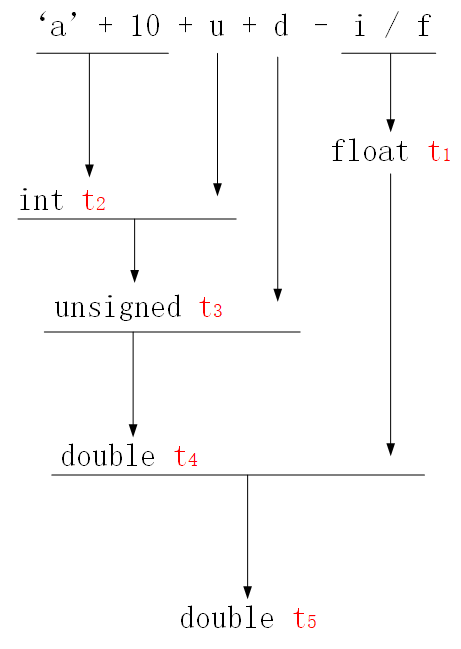
\includegraphics[width=0.7\textwidth]{biaodashi.png}
\end{figure}
\end{yellowblock}
\end{columns}
\end{frame}

%---------------------------------------------------------------------------------------------
\begin{frame}[fragile]{2.5 表达式\normalsize{~---~赋值运算符}}
\begin{columns}[t]
\column{0.5\textwidth}
\begin{block}{赋值运算符:=}
格式:\alert{对象 = 表达式}\\
\begin{lstlisting}
例如
int i = 2;  //对象的初始化
i = 5;      //对象的赋值
i = i + 6;  //对象的赋值
\end{lstlisting}
\end{block}

\column{0.45\textwidth}
\begin{block}<2->{}
~\\
\begin{itemize}
\begin{spacing}{1.35}
  \item 优先级:\textcolor{red}{赋值运算符}<算术运算符
  \item 结合性:\alert{右结合}
  \item 结果:\alert{左值}(C语言是右值)
\end{spacing}
\end{itemize}

\end{block}
\end{columns}

\begin{yellowblock}<3->{说明}
\begin{itemize}
  \item 功能是把赋值符号右侧表达式的值写入到赋值符号左侧的操作对象里面
  \item 左侧操作对象必须是支持写操作的左值,例如\begin{lstlisting}
int i = 0, j = 2;
i + j = 10;//错误:算术表达式为右值
\end{lstlisting}
\end{itemize}
\end{yellowblock}
\end{frame}

%---------------------------------------------------------------------------------------------
\begin{frame}[fragile]{2.5 表达式\normalsize{~---~赋值运算符}}
\begin{redblock}{注意}
\begin{itemize}
\pause
    \item 对象的初始化不是赋值操作,赋值是对象已经定义的情况下,赋一个新值
\pause
    \item 两侧的操作对象的类型不相同,会进行类型转换,但右侧本身的不会发生变化,如  \vspace{-2mm}
\pause
\begin{lstlisting}
int i = 0;
double d = 3.14159;
i = d; //表达式的结果的类型是 int,值是3,但d的值不变
\end{lstlisting} \vspace{-2mm}
\pause
    \item 赋值运算满足右结合性,例如
\pause \vspace{-2mm}
\begin{lstlisting}
i = j = 5; //i 和 j 的值都是5
//根据右结合性,先把 5 赋给 j ,然后把 j = 5 的值赋给 i。
\end{lstlisting} \vspace{-2mm}
\pause
    \item 赋值运算符的优先级是较低,有时需要加上括号才能正确执行,例如:
\pause \vspace{-2mm}
\begin{lstlisting}
i = 2 + j = 4; //错误:2 + j 为右值,不能作为第二个赋值符号的左侧对象
i = 2 + (j = 4); //正确:把 j = 4 的值加上2赋给 i , i 和 j 的值分别为6和4
\end{lstlisting}
 \vspace{-2mm}
\end{itemize}
\end{redblock}
\end{frame}

%---------------------------------------------------------------------------------------------
\begin{frame}[fragile]{2.5 表达式\normalsize{~---~赋值运算符}}

\begin{columns}[t]
\column{0.4\textwidth}
\begin{blueblock}{代码示例}
\begin{lstlisting}
int counter;
counter = counter + 5;
\end{lstlisting}
\end{blueblock}

\begin{blueblock}<3->{例如}
\begin{lstlisting}
counter += 1;
//等效于 counter = counter + 1;
//且只需计算一次,提高了计算效率
i *= j + 3;
//等效于 i = i * (j + 3);
\end{lstlisting}
\end{blueblock}

\column{0.45\textwidth}
\begin{yellowblock}<2->{代码分析}
第二行代码需要进行两次计算,首先计算(\texttt{couter+5})的值,然后再赋值给\texttt{counter}。为简化计算,\texttt{C++}提供了\alert{复合运算符(\texttt{+=}~~~\texttt{-=}~~~\texttt{/=}~~~\texttt{*=}~~~\texttt{\%=})}
\end{yellowblock}

\begin{yellowblock}<4->{小结}
使用复合赋值运算符能够提高运算效率,减少了产生临时对象这一环节
\end{yellowblock}
\end{columns}
\end{frame}

%---------------------------------------------------------------------------------------------
\begin{frame}[fragile]{2.5 表达式\normalsize{~---~自增自减运算符}}
\begin{columns}[t]
\column{0.6\textwidth}
观察如下代码
\begin{blueblock}{代码示例}
\begin{lstlisting}
int i = 5, j = 6;
i += 1;
j -= 1;
\end{lstlisting}
\end{blueblock}

\begin{blueblock}<3->{例如}
\begin{lstlisting}
int i = 0, j;
j = i++;
//后置,i的值自增变为1,表达式 i++ 的值为 i 自增之前的值,即 j 的值为0
j = ++i;
//前置,i的值自增变为2,表达式 ++i 的值为 i 自增之后的值,即 j 的值为2
\end{lstlisting}
\end{blueblock}

\column{0.35\textwidth}
\begin{block}<2->{}
~\\
\begin{spacing}{1.5}
为简化自增1和自减1操作,\texttt{C++}提供了\alert{自增\texttt{(++)}}~和\alert{自减\texttt{(--)}}~运算符
\end{spacing}
\end{block}

\begin{redblock}<4->{注意}
\begin{itemize}
  \item 自增、自减运算符的操作对象必须为左值
  \item 前置版本返回左值对象本身,后置版本将原始值的副本作为右值返回
  \item 建议能用前置版本不用后置版本
\end{itemize}
\end{redblock}
\end{columns}
\end{frame}

%---------------------------------------------------------------------------------------------
\begin{frame}[fragile]{2.5 表达式\normalsize{~---~逻辑和关系运算符}}
\begin{columns}[t]
\column{0.4\textwidth}

\begin{table}[h]
\begin{center}
\small
\textcolor{blue}{逻辑和关系运算符}
~\\
~\\
{\scalebox{0.9}{
\renewcommand\arraystretch{1.5}
\begin{tabular}{cccc}\arrayrulecolor{darkblue}
\hline
\rowcolor{lightblue}运算符&功能&结合性&用法\\
\hline
\texttt{!}& 逻辑非&右&	\texttt{!}5\\
\hline
\texttt{<}&	小于&左&	  5\texttt{<}4\\
\texttt{<=}&小于等于&左&	5\texttt{<=}4\\
\texttt{>}&	大于&左&	5\texttt{>}4\\
\texttt{>=}&大于等于&左&	5\texttt{>=}4\\
\hline
\texttt{==}&等于&左&	5\texttt{==}4\\
\texttt{!=}&不等于&左&	5\texttt{!=}4\\
\hline
\texttt{\&\&}&逻辑与&左&	5\texttt{\&\&}4\\
\hline
\texttt{||}&逻辑或&左&	5\texttt{||}4\\
\hline
\end{tabular}}}
\end{center}
\end{table}
\pause
\column{0.5\textwidth}
~\\
~\\
~\\
\begin{block}{ }
\begin{spacing}{1.}
优先级:\\
赋值运算符~\texttt{<}~~\textcolor{blue}{逻辑或\texttt{||}~<~ 逻辑与\texttt{\&\&}~}~\texttt{<}~\textcolor{red}{关系运算符}~\texttt{<}~算术运算符~\texttt{<}~\textcolor{blue}{逻辑非\texttt{!}}
\end{spacing}
\end{block}
\pause
\begin{block}{ }
\begin{spacing}{1.}
关系运算符内部优先级:\\
\texttt{==}~和~\texttt{!=}~\alert{低于}~\texttt{<=}、\texttt{>}~和 ~\texttt{>=}\\
\end{spacing}

\end{block}

\begin{block}{ }
\begin{spacing}{1.}
结果:右值
\end{spacing}

\end{block}

\end{columns}
\end{frame}

%---------------------------------------------------------------------------------------------
\begin{frame}[fragile]{2.5 表达式\normalsize{~---~逻辑和关系运算符}}
\begin{center}
可以用\texttt{~i~$<=$~j~$<=$~k}直接\alert{构造表达式}\texttt{$i\leq j\leq k$}的逻辑关系吗?
\end{center}
\pause
\begin{columns}[t]
\column{0.9\textwidth}
\begin{greenblock}<2->{答案}
~\\
    \begin{spacing}{1.5}
不能,因为只要 k 大于等于1,表达式\texttt{~i~$<=$~j~$<=$~k}的值永远为真,应该使用逻辑与 \texttt{\&\&}构造表达式,即:\texttt{i <= j \texttt{\&\&} j <= k}
    \end{spacing}
\end{greenblock}
\end{columns}
\end{frame}

%---------------------------------------------------------------------------------------------
\begin{frame}[fragile]{2.5 表达式\normalsize{~---~逻辑和关系运算符}}
\begin{columns}[t]
\column{0.45\textwidth}
给出以下代码运行后\texttt{j}和\texttt{b}的值
\begin{blueblock}{示例代码}
\begin{lstlisting}
int i = 1, j = 2;
bool b = !i && ++j;
\end{lstlisting}
\end{blueblock}

\column{0.25\textwidth}
~\\
~\\
\begin{greenblock}<2->{答案}
\texttt{j=2, b=0}
\end{greenblock}
\end{columns}

\begin{columns}[t]
\column{0.8\textwidth}
\begin{yellowblock}<3->{\texttt{\&\&}和\texttt{||}运算符的运算规则}
\textcolor{red}{逻辑与\texttt{\&\&}}和\textcolor{red}{逻辑或\texttt{||}}运算符都是先计算左侧对象的值,然后根据左侧对象的值判断是否计算右
侧运算对象的值,即为\alert{短路求值}
\begin{itemize}
  \item \texttt{\&\&},仅当左侧运算对象的值为真时,才计算右侧运算对象的值
  \item \texttt{||},仅当左侧运算对象的值为假时,才计算右侧运算对象的值
\end{itemize}
\end{yellowblock}
\end{columns}
\end{frame}

%---------------------------------------------------------------------------------------------
\begin{frame}[fragile]{2.5 表达式\normalsize{~---~逻辑和关系运算符}}
\begin{columns}[t]
\column{0.8\textwidth}

已知\texttt{int a=10, b=20, c=30; float x=1.8, y=2.4;}\\求解\texttt{a<b\texttt{\&\&}x>y\texttt{||}a<b-!c}
\pause
%\textcolor{blue}{答案:}
\end{columns}
\begin{columns}[t]
\column{0.55\textwidth}
\begin{yellowblock}{}
\begin{figure}[!h]
\centering
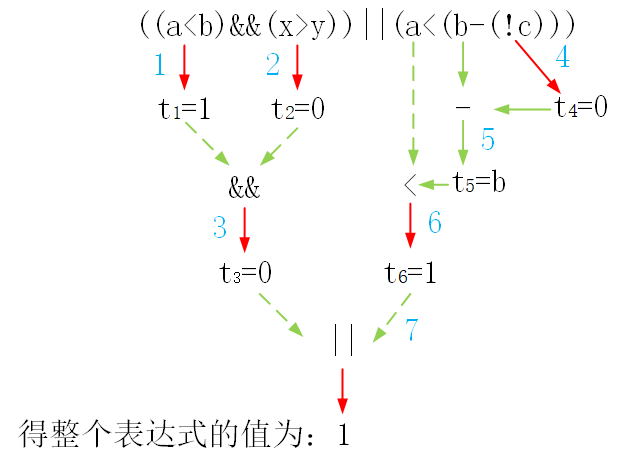
\includegraphics[width=0.9\textwidth]{luoji.png}
\end{figure}
\end{yellowblock}
\end{columns}
\end{frame}

%---------------------------------------------------------------------------------------------
\begin{frame}[fragile]{2.5 表达式}
\begin{center}
  \textcolor{blue}{练习}
\end{center}
\begin{spacing}{1.5}
1.已知\texttt{int a=1,b=5,c=2,d=6;}求解下列表达式及相应对象的的值\\
\begin{tabular}{lll}
  % after \\: \hline or \cline{col1-col2} \cline{col3-col4} ...
  (1)\texttt{a+b>c+d} & (2)\texttt{a=(b=4)+(c=6)} &(3)\texttt{a+=c=b*a} \\
   (4)\texttt{d=(a++)-(++b)+c--} &  (5)\texttt{--a||b<d\&\&c--} & ~ \\
\end{tabular}

2.逻辑表达式的构造:\texttt{a}和\texttt{b}之一为\texttt{0},但不同时为\texttt{0}\\
\pause
\textcolor{blue}{
1.(1)表达式的值为0, \texttt{a,b,c,d}不变\\
~~~(2)表达式的值为10,\texttt{a=10,b=4,c=6}\\
~~~(3)表达式的值为6,\texttt{a=6,b=5,c=5}\\
~~~(4)表达式的值为-3,\texttt{a=2,b=6,c=1,d=-3}\\
~~~(5)表达式的值为1,\texttt{a=0,b=5,c=1,d=6}\\
2.答案一:\texttt{a==0\texttt{\&\&}b\texttt{!}=0\texttt{||}a\texttt{!}=0\texttt{\&\&}b==0}等价于\texttt{!a\&\&b||a\&\&!b}\\
~~~答案二:\texttt{a*b==0\texttt{\&\&}a+b\texttt{!}=0}\\
}
\end{spacing}
\end{frame}


%---------------------------------------------------------------------------------------------
\begin{frame}[fragile]{2.5 表达式\normalsize{~---~逗号运算符}}
逗号表达式:由逗号运算符连接起来的表达式。\alert{从左向右}依次计算每个运算对象,结果为\alert{最右边}的运算对象
\begin{columns}[t]
\column{0.32\textwidth}
\begin{blueblock}{格式如下}
\begin{lstlisting}
exp1, exp2, ...
\end{lstlisting}
\end{blueblock}
\begin{blueblock}<2->{例如}
\begin{lstlisting}
int i, j;
i = (j=3, j+=6, 5+6);
// i 的值为11, j 的值为9
\end{lstlisting}
\end{blueblock}
\column{0.63\textwidth}
\begin{block}<3->{ }
\begin{spacing}{1.2}
优先级:\\
\alert{逗号运算符}\texttt{<}赋值运算符\texttt{<}关系运算符\texttt{<}算术运算符
\end{spacing}
\end{block}
\begin{yellowblock}<4->{说明}
\begin{itemize}
  \item 逗号表达式的值是最右边表达式的值
  \item 在所有的运算符中,逗号运算符的优先级最低
\end{itemize}
\end{yellowblock}
\end{columns}
\end{frame}

%---------------------------------------------------------------------------------------------
\begin{frame}[fragile]{2.5 表达式\normalsize{~---~条件运算符}}
\begin{columns}[t]
\column{0.4\textwidth}
\begin{blueblock}{格式如下}
\begin{lstlisting}
cond ? expr1 : expr2
\end{lstlisting}
\end{blueblock}
\pause
\begin{yellowblock}{ }
\begin{figure}[!h]
\centering
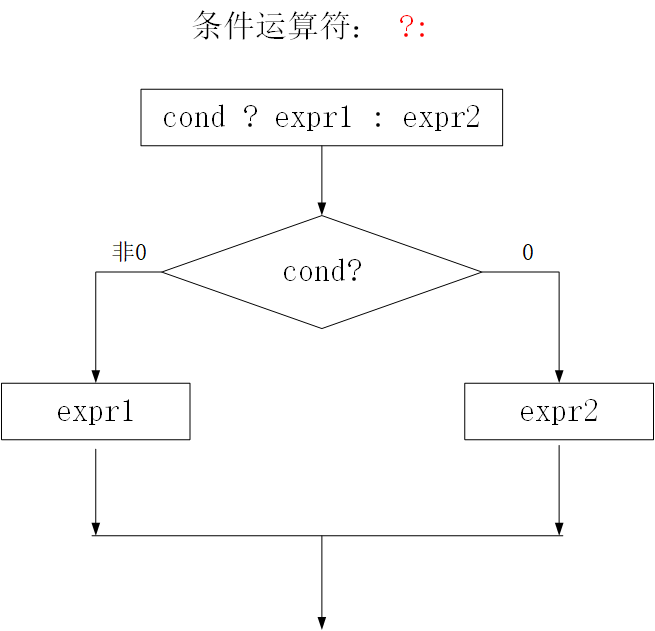
\includegraphics[width=0.8\textwidth]{tiaojian.png}
\end{figure}
\end{yellowblock}
\pause
\column{0.5\textwidth}
\begin{blueblock}{条件运算符允许\alert{嵌套使用},如}
\begin{lstlisting}
int a=4, b=5, c=6, max;
max=a>b?(a>c?a:c):(b>c?b:c);
\end{lstlisting}
\end{blueblock}
\pause
\begin{yellowblock}{建议}
由于会降低程序的可读性,条件运算符不宜嵌套使用
\end{yellowblock}

\pause
\begin{yellowblock}{说明}
条件运算符是唯一的三目运算符
\end{yellowblock}

\end{columns}
\end{frame}

%---------------------------------------------------------------------------------------------
\begin{frame}[fragile]{2.5 表达式\normalsize{~---~sizeof运算符}}
\alert{\texttt{sizeof}运算符}返回一个表达式或一个类型所占内存的字节数
\begin{columns}[t]
\column{0.55\textwidth}
\begin{blueblock}{一般格式}
\begin{lstlisting}
格式:
sizeof (type) 或
sizeof (expr)
例如:
cout << sizeof (int);//输出4
int i=0;
cout << sizeof (++i);//输出4,i 的值为0
\end{lstlisting}
\end{blueblock}
\column{0.4\textwidth}
\begin{redblock}<2->{注意}
\texttt{sizeof(expr)}形式只是返回表达式结果的数据类型的字节数,并不会实际运算表达式,因此左边执行完输出语句后,\texttt{i}的值仍然为\texttt{0}
\end{redblock}
\end{columns}

\end{frame}

%---------------------------------------------------------------------------------------------
\begin{frame}[fragile]{2.5 表达式\normalsize{~---~位运算符}}
\begin{itemize}
  \item<1-> 位运算符:按位反~\verb;~;、{\color<2->{blue}左移~\verb;<<;、右移~\verb;>>;}~、按位与~\texttt{\&}、按位异或~\verb;^;、按位或~\texttt{|} (优先级由高到低)
  \item<3-> 运算的对象是\alert{整型对象},处理二进制数
\end{itemize}

\begin{columns}[t]
\column{0.95\textwidth}
\begin{blueblock}<4->{~~\texttt{short a = 3, b = 5;}}
\begin{center}
\begin{tabular}{cr@{~}r@{}cr@{~}r@{~}cr@{~}r@{~}}
b&\verb;~;&00000000~00000101&&\verb;<<;1&00000000~00000101&&\verb;>>;1&00000000~00000101\\\cline{3-3}\cline{6-6}\cline{9-9}
&&11111111~11111010&&&00000000~00001010&&&00000000~00000010 \\
&&-6&&&10&&&2\vspace{0.3cm}\\
a&&00000000~00000011&&&00000000~00000011&&&00000000~00000011\\
b&\texttt{\&}&00000000~00000101&&\texttt{|}&00000000~00000101&&\verb;^;&00000000~00000101\\\cline{3-3}\cline{6-6}\cline{9-9}
&&00000000~00000001&&&00000000~00000111&&&00000000~00000110\\
&&1&&&7&&&6\vspace{0.3cm}\\
\end{tabular}
\end{center}
\end{blueblock}
\end{columns}

\end{frame}

%---------------------------------------------------------------------------------------------
\begin{frame}[fragile]{2.5 表达式\normalsize{~---~求值次序}}
\alert{~~~~~求值次序}
\begin{columns}[t]
\column{0.45\textwidth}
\begin{blueblock}{示例代码}
\begin{lstlisting}
int i = 0, j;
j = i * 2 + ++i;
\end{lstlisting}
\end{blueblock}

\begin{greenblock}{问题}
是先计算\texttt{++i}还是\texttt{i*2},如果先计算表达式 \texttt{i*2}再计算表达式\texttt{++i},那么结果为\texttt{1};反过来,结果则为\texttt{3} 
\end{greenblock}

\column{0.45\textwidth}

\begin{greenblock}<2->{测试结果}
\begin{itemize}
  \item \texttt{VS}编译器,\texttt{j}的值为\texttt{3}
  \item \texttt{GCC}编译器,\texttt{j}的值为\texttt{1} \footnote{\url{https://rextester.com/l/cpp_online_compiler_gcc}}
\end{itemize}
\end{greenblock}
\begin{yellowblock}<3->{建议}
在复合表达式中,不要出现对同一个对象既读又写的情况,容易出错
\end{yellowblock}
\end{columns}

\end{frame}

%%%%%%%%%%%%%%%%%%%%%%%%%%%%%%%%%%%%%%%%%%%%%%%%%%%%%%%%%%%%%%%%%%%%%%%%%%%%%%%%%%%%%%%%%%%%%%
\section{类型转换}
%%%%%%%%%%%%%%%%%%%%%%%%%%%%%%%%%%%%%%%%%%%%%%%%%%%%%%%%%%%%%%%%%%%%%%%%%%%%%%%%%%%%%%%%%%%%%%

%---------------------------------------------------------------------------------------------
\begin{frame}[fragile]{2.6 类型转换\normalsize{~---~隐式转换}}
    $$\text{类型转换}
    \begin{cases}\text{隐式转换}\\
    \text{显示转换(强制类型转化)}
    \end{cases}$$
\pause

\begin{columns}[t]
\column{0.85\textwidth}
\begin{block}{隐式转换}
	\begin{itemize}
		\item 比int类型小的整型类型提升为较大的整型类型: 'a'+125
		\item 将表达式的值转换为布尔值:  $1+3>4*7$
        \item 初始化过程中,初始值转换成定义对象的类型: double i = 3;
        \item 算术表达式中,运算结果转换为运算对象中最宽(大)的数据类型 : 3.14+2+'a'
	\end{itemize}
\end{block}
\end{columns}
\end{frame}

%---------------------------------------------------------------------------------------------
\begin{frame}[fragile]{2.6 类型转换\normalsize{~---~隐式转换}}

\begin{center}
\textcolor{blue}{混合运算的类型转换规则}\\~\\
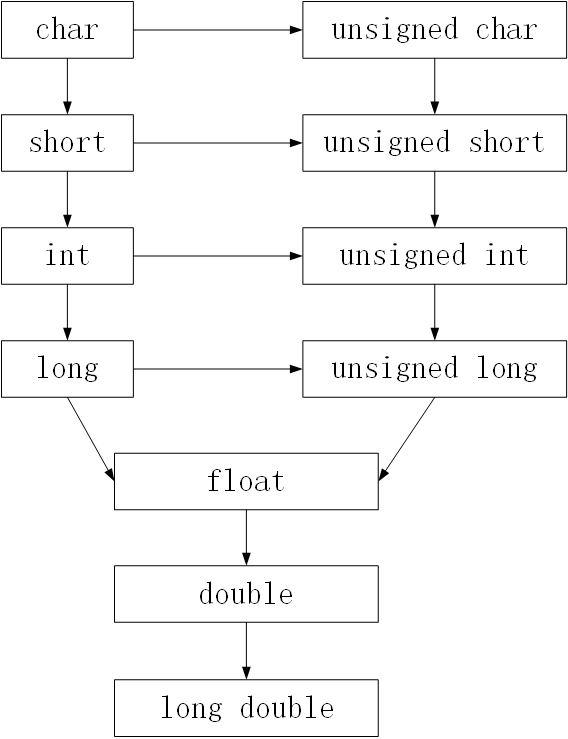
\includegraphics[width=0.3\textwidth]{leixingzhuanhuan.png}
\end{center}


\end{frame}

%---------------------------------------------------------------------------------------------
\begin{frame}[fragile]{2.6 类型转换\normalsize{~---~显示转换}}
显示转换方式:\\
\begin{itemize}
  \item \texttt{\alert{static\_cast}}、\texttt{dynamic\_cast}、\texttt{const\_cast}、\texttt{reinterpret\_cast}
\end{itemize}
\pause
\begin{block}{几种转换方式的应用}
\begin{itemize}
\item \texttt{static\_cast}在算术表达式中的应用
\pause
        \begin{itemize}
          \item 执行浮点数操作,如:\\
          \begin{lstlisting}
int i = 5, j = 3;
double k = i / static_cast<double>(j); //强制将 j 转化为 double 类型
          \end{lstlisting}
\pause
          \item 告诉编译器我们有意将宽类型转换成窄类型,请关闭警告信息,例如:\\
        \begin{lstlisting}
double i = 5., j = 3.;
int k = static_cast<int>(i / j);//强制将 i / j 的结果转化为 int
        \end{lstlisting}
        \end{itemize}
\pause
\item \texttt{const\_cast}常用来去掉对象的 const 属性,即把 const 对象转换为非const对象
\end{itemize}
\end{block}
\end{frame}

%---------------------------------------------------------------------------------------------
\begin{frame}[fragile]{2.6 类型转换\normalsize{~---~显示转换}}
\begin{columns}[t]
\column{0.45\textwidth}
\begin{center}
  \textcolor{blue}{其他的类型转换方式}
\end{center}
\begin{blueblock}{例如}
格式:
        \begin{lstlisting}
type (expr) //函数方式,或者
(type) expr //C语言方式
        \end{lstlisting}
例如:
        \begin{lstlisting}
double k = i / (double)j;
//强制将 j 转化为 double 类型
double k = i / double (j);
        \end{lstlisting}
\end{blueblock}
\pause
\column{0.45\textwidth}
~\\
~\\
~\\
~\\
\begin{yellowblock}{提示}
类型转换不会改变对象本身的值,如:\\
        \begin{lstlisting}
double i = 5.;
int j = i;
//将 i的结果转化为 int,但i的值不变
int k = static_cast<int>(i);
//强制将 i的结果转化为 int,但i的值不变
        \end{lstlisting}
\end{yellowblock}
\end{columns}
\end{frame}


%---------------------------------------------------------------------------------------------
\begin{frame}[fragile]{课后作业}

\begin{columns}[t]
\column{0.8\textwidth}
\begin{blueblock}{作业本}
 \begin{enumerate}
   \item 习题2.2、2.3、2.6、2.10和2.12
 \end{enumerate}

\end{blueblock}

\begin{blueblock}{上机练习}
 \begin{enumerate}
   \item 实验指导书:第二章
 \end{enumerate}

\end{blueblock}
\end{columns}
\end{frame}


%---------------------------------------------------------------------------------------------
\begin{frame}[fragile]
	\frametitle{~~}
	\begin{center}
		\huge{本章结束}
	\end{center}
\end{frame}

\end{document}

\end{document}
